\documentclass[answers, 11pt]{exam}

\usepackage[spanish]{babel}
\usepackage[shortlabels]{enumitem}
\usepackage[T1]{fontenc}
\usepackage{graphicx}
\usepackage[cache=false,outputdir=./build]{minted}
\usepackage{lmodern}
\usepackage{wrapfig}
\usepackage{xcolor, color}
\definecolor{LightGray}{gray}{0.9}

\newcommand{\materia}{Analisis de Algoritmos 2024-1}
\newcommand{\tarea}{Tarea 07: Ordenamientos II}
\newcommand{\fecha}{\today}
\newcommand{\profesor}{Profesor(a): María de Luz Gasca Soto}
\newcommand{\ayudantes}{
  Rodrigo Fernando Velázquez Cruz \\
  Teresa Becerril Torres
}
\newcommand{\alumnos}{
  Alvaro Ramirez Lopez \textbf{N° cuenta:} 316276355
}

\decimalpoint{}
\graphicspath{{Imagenes}}
% \colorsolutionboxes
\shadedsolutions

% \definecolor{SolutionBoxColor}{rgb}{0,128,255}
% \definecolor{SolutionColor}{rgb}{0,204,255}
\definecolor{SolutionColor}{rgb}{0,128,255}

\renewcommand{\familydefault}{\sfdefault}

\extrawidth{1.56cm}
\extraheadheight[1.5in]{-0.25in}
\extrafootheight[-0.175in]{-0.375in}
\firstpageheader{
}{
  \begin{minipage}[c]{3.5cm}
    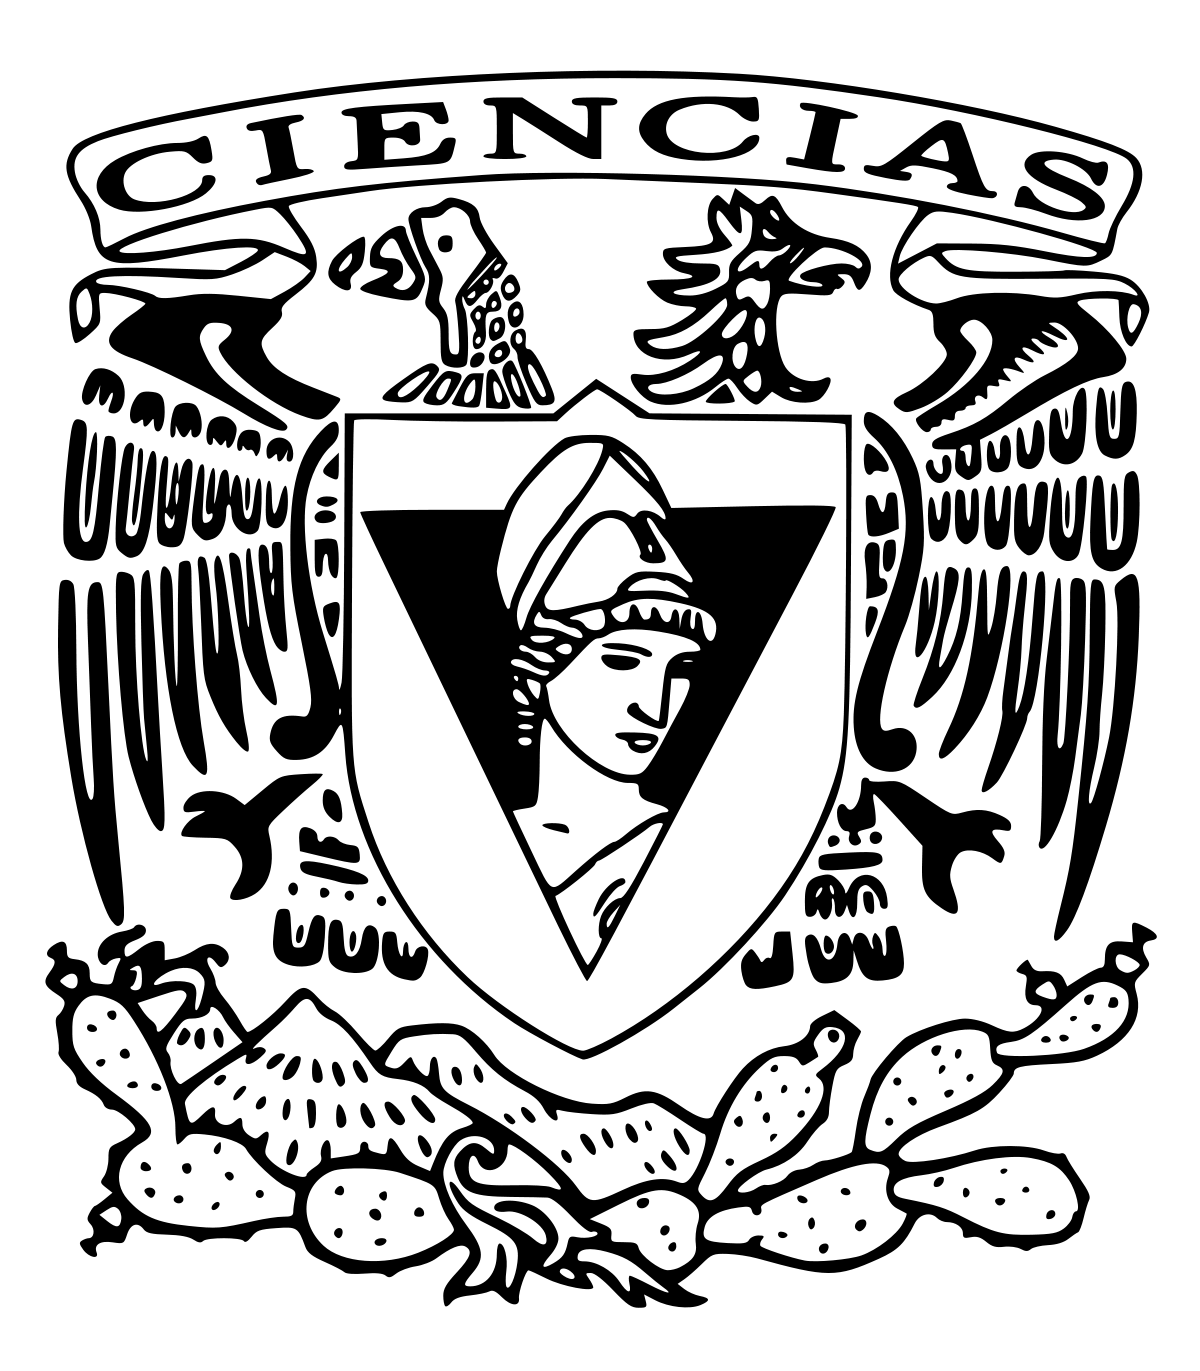
\includegraphics[width=3.5cm]{fc.png}
  \end{minipage}
  \begin{minipage}[c]{11.0cm}
    {\bfseries\huge\materia{} \\[2mm]
      \LARGE \tarea{} \\
      \large Profesor:} \profesor{} \\
    \hspace{0.1cm}
    {\bfseries\large Ayudantes:}
    \begin{minipage}[t]{8.5cm}
      \ayudantes{}\vspace{0.1cm}
    \end{minipage}\hfill\break{}
    {\bfseries\large Alumno:}
    \begin{minipage}[t]{8.5cm}
      \alumnos{}\\
    \end{minipage}\hfill\break{}
  \end{minipage}
  \begin{minipage}[c]{3.25cm}
    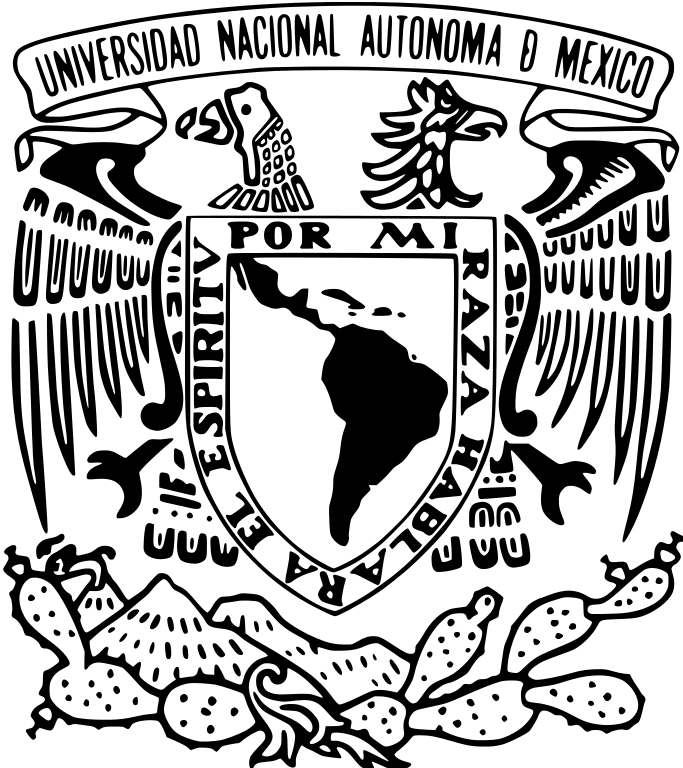
\includegraphics[width=3.25cm]{unam.png}
  \end{minipage}
}{}
\runningheader{\materia}{\tarea}{\fecha}
\runningheadrule{}
\footer{}{Página \thepage\ de \numpages}{}
\footrule{}
\renewcommand{\solutiontitle}{\noindent\textbf{Solución:}\par\noindent}



\begin{document}
\begin{questions}
\question{
El Problema de Seleccion consiste en encontrar el k-esimo elemento
mas pequeño de un conjunto de n datos. Utilizar las estrategias
usadas por el algoritmo \textbf{Quick Sort}, como el proceso Partition, para
resolver el problema de Selección. El algoritmo propuesto deberá tener
desempeño computacional de $O(n)$, en el caso promedio. Justifique
con detalle sus respuestas.
}

\begin{solution}
  Para resolver este problema, primero vamos a tener en cuenta que técnica aplica 
  la función \textit{partición}:
    
    \begin{center}
      \fbox
    {
    \begin{minipage}{0.85\textwidth}
      \textit{Partición(a,b)}: Divide el conjunto de datos en dos subconjuntos, 
      uno con elementos menores o iguales
      al pivote y otro con elementos mayores al pivote.
    \end{minipage}
    }
    \end{center}
    Para resolver el problema de selección, podemos modificar el algoritmo 
    QuickSort para que, en lugar de ordenar todo el conjunto de datos, solo 
    interactuemos con la mitad de los datos, el algoritmo propuesto lo expresaremos
    en \textbf{Lenguaje Python} para que sea más fácil de entender:

    \begin{minted}[
      frame=lines,
      framesep=2mm,
      % baselinestretch=1.2,
      bgcolor=LightGray,
      fontsize=\footnotesize,
      linenos
      ]{Python}
  def select_kth_smallest(arr, k):
    while True:
        # Elegir un pivote de forma aleatoria
        pivot = arr[random.randint(0, len(arr) - 1)]
        
        # Inicializar las listas para elementos menores, iguales y mayores que el pivote
        less = []
        equal = []
        greater = []
        
        # Particionar el arreglo en los tres grupos
        for element in arr:
            if element < pivot:
                less.append(element)
            elif element == pivot:
                equal.append(element)
            else:
                greater.append(element)
        
        # Decidir en cuál de los grupos se encuentra el k-ésimo elemento
        if k < len(less):
            arr = less
        elif k < len(less) + len(equal):
            return pivot
        else:
            k = k - len(less) - len(equal)
            arr = greater
    \end{minted}

    Para justificar el algoritmo, lo mostraremos con 3 puntos:
    \begin{itemize}
      \item \textbf{Eficiencia promedio}: La elección aleatoria del pivote garantiza que, 
      en promedio, se obtendrán divisiones equilibradas en el arreglo en cada 
      iteración. Esto se traduce en un rendimiento promedio de $O(n)$ ya que, en 
      promedio, se reduce a la mitad el tamaño del arreglo en cada iteración.

      \item \textbf{Correctitud}: El algoritmo divide el arreglo en tres grupos: elementos 
      menores que el pivote, iguales al pivote y mayores que el pivote (que serian en el caso 
      recurrente solo 1 elemento). Luego, decide en cuál de estos grupos se encuentra 
      el k-ésimo elemento y se enfoca en ese grupo.
      
      \item \textbf{Partición}: La función Partition se utiliza de manera efectiva para 
      dividir el arreglo en tres grupos en cada iteración. Esto garantiza que el 
      algoritmo se ejecute de manera eficiente y que no se requieran más de $O(n)$ 
      comparaciones en el caso promedio.
    \end{itemize}

    En resumen, utilizando la estrategia de partición modificada y la elección aleatoria del 
    pivote, este algoritmo de selección garantiza un desempeño computacional 
    promedio de $O(n)$ en el caso promedio, lo que lo convierte en una solución 
    eficiente para encontrar el k-ésimo elemento más pequeño en un conjunto de datos.

\end{solution}

\question{
Sea \textbf{QuickSort 1} la versión de \textit{Quick Sort} que toma como pivote al
elemento $A[(first + last) \verb| div | 2]$; y sea Sea \textbf{QuickSort 2} la versión que
toma como pivote al elemento que resulta ser la mediana de $A[first]$, 
$A[(first + last) \verb| div | 2]$, $A[last]$.

Dar un ejemplo de una lista de al menos 23 valores donde el desempeño
computacional de \textbf{QuickSort 2} sea mejor que el de \textbf{QuickSort 1}
}

\begin{solution}
  Ejemplo de lista de 23 valores:

Supongamos que tenemos la siguiente lista de 23 valores, que está preordenada de manera inversa (en orden descendente):

\begin{center}
  \verb|A = [23,22,21,20,19,18,17,16,15,14,13,12,11,10,9,8,7,6,5,4,3,2,1]|
\end{center}

Sabiendo ya como deberemos de tomar los pivotes para los casos de QuickSort 1 y 2, 
comenzaremos a ver como es el comportamiento para ambos casos:

\begin{itemize}
  \item \textbf{QuickSort 1:}
  
  En QuickSort 1, el pivote se selecciona en el medio de la sublista. En este caso, 
  el pivote sería A[11], que tiene un valor de 12. El algoritmo dividirá la lista 
  en dos sublistas: una con elementos mayores que 12 y otra con elementos menores. 
  Esto da como resultado dos sublistas de 11 elementos cada una.

  Después de la primera partición, tenemos algo como esto:
  \begin{center}
    \verb|A = [23,22,21,20,19,18,17,16,15,14,13] [12] [11,10,9,8,7,6,5,4,3,2,1]|
  \end{center}

  Ahora veremos las demás llamadas

  \verb|Pivote = A[11] = 12|. 
  
  \begin{enumerate}
    \item Dividimos la lista en dos sublistas: elementos mayores que 12 y elementos menores que 12.

    [23, 22, 21, 20, 19, 18, 17, 16, 15, 14, 13] | 12 | [11, 10, 9, 8, 7, 6, 5, 4, 3, 2, 1]
  
    Sublista izquierda:
  
    
    [23, 22, 21, 20, 19, 18, 17, 16, 15, 14, 13]
    
  
    Sublista derecha:
  
    
    [11, 10, 9, 8, 7, 6, 5, 4, 3, 2, 1]
    
  
  \item Ahora aplicamos QuickSort 1 en ambas sublistas.
  
    Sublista izquierda:
  
    Pivote = `A[5] = 18`. Dividimos la sublista izquierda en dos sublistas:
    
    [23, 22, 21, 20, 19] | 18 | [17, 16, 15, 14, 13]
  
    Sublista izquierda (18 y menores):
    
    [17, 16, 15, 14, 13]  
  
    Sublista derecha (mayores que 18):
  
    [23, 22, 21, 20, 19]
  
    Sublista derecha:
  
    Pivote = `A[5] = 6`. Dividimos la sublista derecha en dos sublistas:
    
    [11, 10, 9] | 8 | [7, 6, 5, 4, 3, 2, 1]
  
    Sublista izquierda (8 y menores):
  
    [7, 6, 5, 4, 3, 2, 1]
    
    Sublista derecha (mayores que 8):
    
    [11, 10, 9]
  
    \item Continuamos aplicando QuickSort 1 en todas las sublistas. Las sublistas que solo tienen un elemento ya están ordenadas y no requieren más divisiones.
  \end{enumerate}

   El proceso continúa hasta que todas las sublistas estén ordenadas.

  \item \textbf{QuickSort 2:}
  En QuickSort 2, el pivote se selecciona como la mediana de los elementos en 
  las posiciones \verb|first, (first + last) div 2|, y \verb|last|. Para esta lista, eso 
  significa que el pivote es el valor 12 (la mediana de 23, 12, y 1).

  \begin{enumerate}
    \item Pivote = Mediana de 23, 12 y 1 = 12. Dividimos la lista en dos sublistas de igual tamaño:

    
    [23, 22, 21, 20, 19, 18, 17, 16, 15, 14, 13] | 12 | [11, 10, 9, 8, 7, 6, 5, 4, 3, 2, 1]
    
    \item Aplicamos QuickSort 2 en ambas sublistas.
    
    Sublista izquierda:
    
    [23, 22, 21, 20, 19, 18, 17, 16, 15, 14, 13]
    
    Sublista derecha:
    
    [11, 10, 9, 8, 7, 6, 5, 4, 3, 2, 1]
    
    \item Pivote en la sublista izquierda = Mediana de 23, 18 y 13 = 18. Dividimos la sublista izquierda en dos sublistas:
    
    [23, 22, 21] | 18 | [17, 16, 15, 14, 13]
    
    Sublista izquierda:
    
    [23, 22, 21]
    
    Sublista derecha:
    
    [17, 16, 15, 14, 13]
    
    Sublista derecha:

    Pivote = `A[2] = 21`. Dividimos la sublista derecha en dos sublistas:

    [17, 16, 15] | 14 | [13]
    
    Sublista izquierda:
    
    [17, 16, 15]
    
    Sublista derecha:

    [13]
    
    La sublista derecha ya está ordenada y no requiere más divisiones.

 \item Continuamos aplicando QuickSort 2 en todas las sublistas. El proceso continúa hasta que todas las sublistas estén ordenadas.
  \end{enumerate}

\end{itemize}

\end{solution}

\question{
Proporcione una secuencia $L$ de enteros diferentes, de tres dígitos cada
uno. Considere $|L| \geq 30$
Aplique \textbf{Bucket Sort} a $L$ de dos maneras distintas.
}

\begin{solution}
  Supongamos que tenemos la siguiente secuencia de números de tres dígitos:
    \begin{verbatim}
      L = [721, 189, 355, 532, 482, 658, 846, 124, 906, 299, 773, 675, 
      231, 543, 916, 102, 418, 587, 367, 894, 766, 159, 618, 437, 903, 
      279, 683, 526, 135, 718, 490]  
    \end{verbatim}
  Primero, aplicaremos el Bucket Sort de una manera:

  \textbf{Bucket Sort primera forma:}
  \begin{enumerate}
    \item Creamos una lista de 10 cubos, uno para cada dígito (0-9) que corresponda a cada centena de $L$.
    \begin{verbatim}
      Cubo_0: []
      Cubo_1: []
      Cubo_2: []
      Cubo_3: []
      Cubo_4: []
      Cubo_5: []
      Cubo_6: []
      Cubo_7: []
      Cubo_8: []
      Cubo_9: []
    \end{verbatim}
    \item Colocamos cada número de la secuencia L en el cubo correspondiente según su dígito de las centenas.
    \begin{verbatim}
      Cubo_0: []
      Cubo_1: [189, 124, 102, 159, 135]
      Cubo_2: [299, 231, 279]
      Cubo_3: [355, 367]
      Cubo_4: [482, 418, 437, 490]
      Cubo_5: [532, 543, 587, 526]
      Cubo_6: [658, 675, 618, 683]
      Cubo_7: [721, 773, 766, 718]
      Cubo_8: [846, 894]
      Cubo_9: [906, 916, 903]
    \end{verbatim}
    \item Ordenamos cada cubo individualmente, por ejemplo, con QuickSort Sort.
    \begin{verbatim}
      Cubo_0: []
      Cubo_1: [102, 124, 135, 159, 189]
      Cubo_2: [231, 279, 299]
      Cubo_3: [355, 367]
      Cubo_4: [418, 437, 482, 490]
      Cubo_5: [526, 532, 543, 587]
      Cubo_6: [618, 658, 675, 683]
      Cubo_7: [718, 721, 766, 773,]
      Cubo_8: [846, 894]
      Cubo_9: [903, 906, 916]
    \end{verbatim}
    \item Concatenamos los cubos ordenados en orden, lo que resulta en la lista ordenada.
    \begin{verbatim}
      lista_ordenada = Cubo_0[] ++ Cubo_1[] ++ Cubo_2[] ++ Cubo_3[] ++ Cubo_4[] 
      ++ Cubo_5[] ++ Cubo_6[] ++ Cubo_7[] ++ Cubo_8[] ++ Cubo_9[]
    \end{verbatim}
    \item Aplicando esto a la secuencia L, obtendremos la lista ordenada.
    \begin{verbatim}
      lista_ordenada = [102, 124, 135, 159, 189, 231, 279, 299,
      355, 367, 418, 437, 482, 490, 526, 532, 543, 587, 618, 658,
      675, 683, 718, 721, 766, 773, 846, 894, 903, 906, 916]
    \end{verbatim}
  \end{enumerate}

  Ahora, vamos a aplicar el Bucket Sort de segunda manera:
  
  \textbf{Bucket Sort de segunda manera:}
  \begin{enumerate}
    \item En lugar de tener solo 10 cubos, creamos un número de cubos igual al número de elementos en la secuencia L.
    \begin{verbatim}
      Cubo_721: []
      Cubo_189: []
      Cubo_355: []
      Cubo_532: []
      Cubo_482: []
      Cubo_658: []
      Cubo_846: []
      Cubo_124: []
      Cubo_906: []
      Cubo_299: []
      Cubo_773: []
      Cubo_675: []
      Cubo_231: []
      Cubo_543: []
      Cubo_916: []
      Cubo_102: []
      Cubo_418: []
      Cubo_587: []
      Cubo_367: []
      Cubo_894: []
      Cubo_766: []
      Cubo_159: []
      Cubo_618: []
      Cubo_437: []
      Cubo_903: []
      Cubo_279: []
      Cubo_683: []
      Cubo_526: []
      Cubo_135: []
      Cubo_718: []
      Cubo_490: []
    \end{verbatim}
    \item Colocamos cada número de la secuencia $L$ en el cubo correspondiente según su valor, es decir, 721 va al cubo 721, 189 va al cubo 189, etc.
    \begin{verbatim}
      Cubo_721: [721]
      Cubo_189: [189]
      Cubo_355: [355]
      Cubo_532: [532]
      Cubo_482: [482]
      Cubo_658: [658]
      Cubo_846: [846]
      Cubo_124: [124]
      Cubo_906: [906]
      Cubo_299: [299]
      Cubo_773: [773]
      Cubo_675: [675]
      Cubo_231: [231]
      Cubo_543: [543]
      Cubo_916: [916]
      Cubo_102: [102]
      Cubo_418: [418]
      Cubo_587: [587]
      Cubo_367: [367]
      Cubo_894: [894]
      Cubo_766: [766]
      Cubo_159: [159]
      Cubo_618: [618]
      Cubo_437: [437]
      Cubo_903: [903]
      Cubo_279: [279]
      Cubo_683: [683]
      Cubo_526: [526]
      Cubo_135: [135]
      Cubo_718: [718]
      Cubo_490: [490]
    \end{verbatim}
    \item Los cubos contienen un solo elemento, por lo que ya están ordenados en sí mismos.
    \item Concatenamos los cubos en orden, lo que resulta en la lista ordenada.
    \begin{verbatim}
      lista_ordenada = Cubo_102[] ++ Cubo_124[] ++ Cubo_135[] ++ Cubo_159[] 
      ++ Cubo_189[] ++ Cubo_231[] ++ Cubo_279[] ++ Cubo_299[] ++ Cubo_355[] 
      ++ Cubo_367[] ++ Cubo_418[] ++ Cubo_437[] ++ Cubo_482[] ++ Cubo_490[] 
      ++ Cubo_526[] ++ Cubo_532[] ++ Cubo_543[] ++ Cubo_587[] ++ Cubo_618[] 
      ++ Cubo_658[] ++ Cubo_675[] ++ Cubo_683[] ++ Cubo_718[] ++ Cubo_721[] 
      ++ Cubo_766[] ++ Cubo_773[] ++ Cubo_846[] ++ Cubo_894[] ++ Cubo_903[] 
      ++ Cubo_906[] ++ Cubo_916[]

      lista_ordenada = [102, 124, 135, 159, 189, 231, 279, 299,
      355, 367, 418, 437, 482, 490, 526, 532, 543, 587, 618, 658,
      675, 683, 718, 721, 766, 773, 846, 894, 903, 906, 916]
    \end{verbatim}
  \end{enumerate}
\end{solution}

\question{
Proporcione una secuencia $L$ de enteros diferentes, en hexadecimal, de
cuatro cifras cada uno. Considere $|L| \geq 25$
\begin{enumerate}[a)]
  \item Ordena la secuencia usando...
  \begin{enumerate}[i)]
    \item ... MSD-Radix-Sort;
    \item ... LSD-Radix-Sort;
  \end{enumerate}
  \item Comente sobre las ejecuciones
\end{enumerate}
}

\begin{solution}
  Aqui va la respuesta
\end{solution}

\question{
\textbf{Opcional} Sea $L$ una lista de $n$ números enteros diferentes. Suponga
que los elementos $x$ de $L$ están en el intervalo $[1, 500]$.
Diseñe un algoritmo de orden lineal que ordene los elementos de $L$.
}

\begin{solution}
  El algoritmo pensado funcionaria de la siguiente manera:
  \begin{enumerate}
    \item Crea un arreglo de conteo count de longitud 500, inicializado con ceros.
    \item Recorre la lista original y para cada elemento num, incrementa el valor en \verb|count[num - 1]| en 1.
    \item Reconstruye la lista ordenada \verb|sorted_arr| a partir del arreglo 
    de conteo, agregando cada numero repetidamente según su frecuencia en el arreglo de conteo.
  \end{enumerate}

  El algoritmo en \textbf{Lenguaje Python} se vería de la siguiente manera:

  \begin{minted}[
    frame=lines,
    framesep=2mm,
    % baselinestretch=1.2,
    bgcolor=LightGray,
    fontsize=\footnotesize,
    linenos
    ]{Python}
  def op_sort(arr):
    # Inicializar un arreglo de conteo con 500 elementos (índices 0-499)
    count = [0] * 500

    # Contar la frecuencia de cada elemento en la lista
    for num in arr:
        count[num - 1] += 1

    # Reconstruir la lista ordenada a partir del arreglo de conteo
    sorted_arr = []
    for i in range(500):
        sorted_arr.extend([i + 1] * count[i])

    return sorted_arr
  \end{minted}

  Para probarlo, podemos declarar en el mismo archivo una lista de 500 elementos y ejecutar el algoritmo, a continuacion 
  se muestra un ejemplo con un arreglo de 10 elementos:

  \begin{minted}[
    frame=lines,
    framesep=2mm,
    % baselinestretch=1.2,
    bgcolor=LightGray,
    fontsize=\footnotesize,
    linenos
    ]{Python}
  def op_sort(arr):
    # Inicializar un arreglo de conteo con 500 elementos (índices 0-499)
    count = [0] * 500

    # Contar la frecuencia de cada elemento en la lista
    for num in arr:
        count[num - 1] += 1

    # Reconstruir la lista ordenada a partir del arreglo de conteo
    sorted_arr = []
    for i in range(500):
        sorted_arr.extend([i + 1] * count[i])

    return sorted_arr

    # Ejemplo de uso:
    lista = [354, 23, 126, 98, 354, 1, 7, 249, 500, 55]
    sorted_lista = op_sort(lista)
    print(sorted_lista)
  \end{minted}
  Eso nos devuelve el arreglo ordenado:
  \begin{center}
    \verb|[1, 7, 23, 55, 98, 126, 249, 354, 354, 500]|
  \end{center}

\end{solution}
  
\end{questions}
\end{document}

